%begin{figure}[!h]
%\begin{minipage}{.5\textwidth}
 % \centering
  %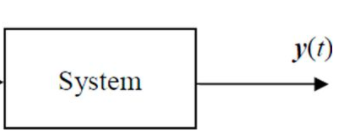
\includegraphics[width=.7\linewidth]{ts_system}
%\end{minipage}%
 % \begin{minipage}{.5\textwidth}
  %\centering
  %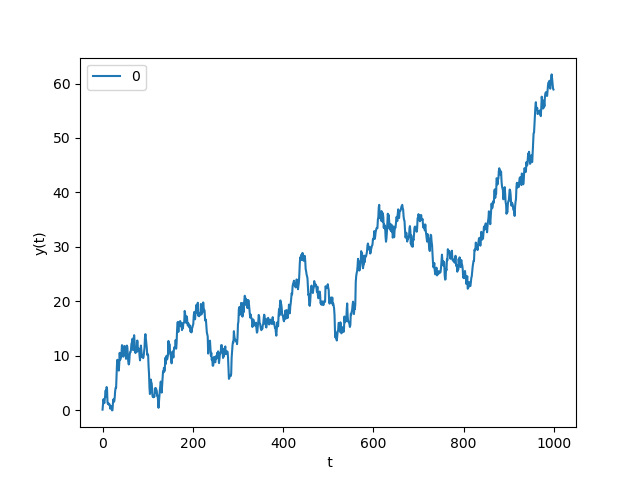
\includegraphics[width=.7\linewidth]{ts}
%\end{minipage}%
%\end{figure}
\section{Chapter 2 : Analysis of Stochastic Processes}
TS modelled with ARMA processes and I/O modelled with ARMAX models can be represented in 4 different ways : 
\begin{itemize}
\item Time domain (Chap.1)
\item Transfer function (Chap.1)
\item \textbf{Probabilistic representation}
\item \textbf{Frequency representation}
\end{itemize}
\subsection{Probabilistic Representation}
\subsubsection{Probabilistic representation of MA(n)}
Time domain representation : $y(t) = c_0e(t)+...+c_ne(t-n), e(t) \sim WN(0,\lambda^2)
$.\\
The process is \textbf{stationary} as all the poles are in the origin.\\
\begin{itemize}
\item \textbf{Mean of y}\\
$$ m_y = E[y(t)] =  E[c_oe(t)+ ...+ c_ne(t-n)] = c_0E[e(t)]+...+c_nE[e(t-n)] $$ 
Because of stationary property $E[e(t)] =...=E[e(t-n)] = 0 $ 
\[
\boxed{m_y=0}
\]

\item \textbf{Covariance of y}
\begin{itemize}
\item $\tau = 0 $\\
$ \gamma_y(0) = E[(y(t)-m_y)^2] = E[y(t)^2]=E[(c_0e(t)+...+c_ne(t-n))^2] =$
$ c_0^2E[e(t)^2]+...+c_n^2E[e(t-n)^2] +2c_0c_1E[e(t)e(t-1)+...+2c_{n-1}c_nE[e(t-n-1)e(t-n)]$ \\where \\$ E[e(t)^2] = E[e(t-1)^2] =...=E[e(t-n)^2] = \lambda^2$ \\ $ E[e(t)e(t-1)]... = 0$ because not correlated \\
\[
\boxed{\gamma_y(0) = \lambda^2(c_0^2 + ...+c_n^2)}
\]
\item $\tau = 1$\\
$ \gamma_y(1)= E[(y(t)-m_y)(y(t-1)-m_y)]=E[y(t)y(t-1)]$ \\ $ E[(c_0e(t)+...+e_ne(t-n))(c_0e(t-1)+...+c_ne(t-n-1)] $ \\ only terms at same time survive : \\ 
$ c_0c_1E[e(t-1)^2]+...+c_{n-1}c_nE[e(t-n)^2] $ \\ where $E[e(t-i)^2] = \lambda^2$ \\ \[
\boxed{\gamma_y(1)= (c_0c_1+c_1c_2+...+c_{n-1}c_n)\lambda^2 }
\]
\item $\tau =2$\\
\[ 
\boxed{\gamma_y(2) = (c_0c_2+c_1c_3+...+c_{n-2}c_n)\lambda^2 }
\]
\item ...\\
\item $\tau = n$\\
\[
\boxed{\gamma_y(n) = c_0c_n\lambda^2}
\]
\item $ |\tau| > n $\\
\[
\boxed{\gamma_y(\tau) = 0 , \tau > n}
\]
Which means that \textbf{MA(n)} has a \textbf{finite memory} of n steps
\end{itemize}
\end{itemize}

\subsubsection{Probabilistic representation of AR(1)}
$y(t) = ay(t-1)+e(t) , e(t) \sim WN(0,\lambda^2)$ \\
Is $y(t)$ a \textbf{SSP}?\\
\textbf{TF representation}:\\
$ y(t) = aZ^{-1}y(t)+e(t) \to y(t) = \frac{1}{1-aZ^{-1}}e(t) \to y(t)=\frac{Z}{Z-a}e(t) $\\
So  $y(t)$ is a SSP if and only if $|a|<1$
\begin{itemize}
\item \textbf{Mean of y}\\
$m_y = E[y(t)] = E[ay(t-1)+e(t)] = am_y + m_e $ \\ 
$m_y(1-a) = m_e  \to m_y = \frac{m_e}{1-a} $ \\ 
$m_e = 0$ so : \\
\[
\boxed{m_y = 0}
\] 
This hold only if the general input $v(t)$ has $m_v = 0$ and the system \textbf{W(Z)} is \textbf{asymptotically stable}.
\item \textbf{Covariance of y}\\
\begin{itemize}
\item $\tau=0$\\
$ \gamma_y(0) = E[(y(t) -m_y)^2] = E[y(t)^2] = E[(ay(t-1)+e(t))^2]$\\
$ \gamma_y(0) = a^2E[y(t-1)^2]+E[e(t)]+2aE[e(t)y(t-1)]$ \\
$ \gamma_y(0) = a^2\gamma_y(0) + \lambda^2 + 0 $ \\
\textbf{Observation: } the fact that $E[e(t)y(t-1)] = 0$ is explained in 2.1.3! \\
\[
\boxed{\gamma_y(0) = \frac{\lambda^2}{1-a^2}}
\]
\item $\tau = 1$\\
$ \gamma_y(1) = E[(y(t)-m_y)(y(t-1)-m_y)] = E[(ay(t-1)+e(t))y(t-1)]$ \\
$ \gamma_y(1) = E[ay(t-1)y(t-1)] + E[e(t)y(t-1)] = a\gamma_y(0) + 0$ \\
\textbf{Observation: } the fact that $E[e(t)y(t-1)] = 0$ is explained in 2.1.3! \\
\[
\boxed{\gamma_y(1) = a\gamma_y(0)}
\]
\item ...\\
\item $\tau \neq 0$\\
\[
\boxed{a\gamma_y(\tau-1)}
\]
Which means that \textbf{AR(1)} has an \textbf{infinite memory}.The formula is also known as \textbf{Yule-Walker formula of order 1}
\end{itemize}
\end{itemize}
\newpage
\begin{description}
\item[1.Plot of $\gamma_y(\tau) , 0<a<1$]\hfill\\
\begin{figure}[H]
 \centering
  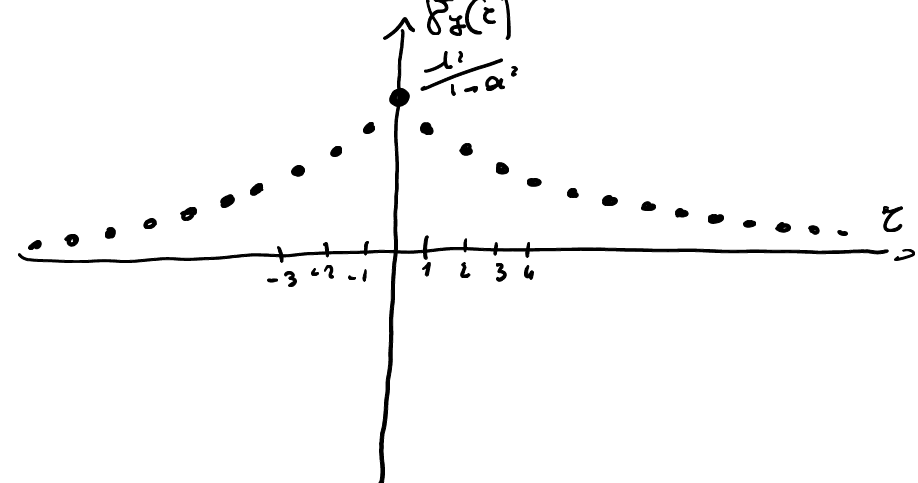
\includegraphics[width=.5\linewidth]{stableplot}
\end{figure}
\item[2.Plot of $\gamma_y(\tau) , -1<a<0$]\hfill\\
\begin{figure}[H]
 \centering
  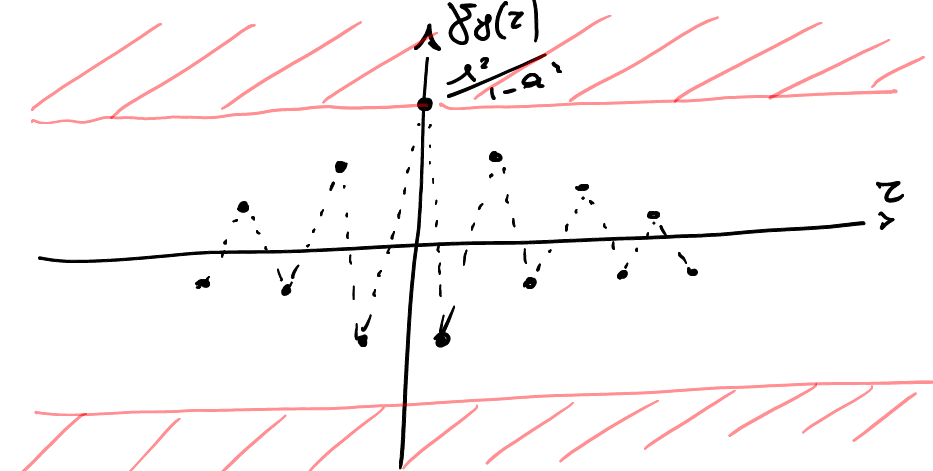
\includegraphics[width=.5\linewidth]{unstableplot}
\end{figure}
\end{description}
\subsubsection{AR/ARMA as MA($\infty$)}
A general rule states that every AR/ARMA stationary stochastic process can be modelled as 	\textbf{MA($\infty$)}. Example with \textbf{AR(1)} as above: \\
$ y(t) = \frac{1}{1-aZ^{-1}}e(t) \to y(t) = \sum\limits_{k=0}^{\infty}(aZ^{-1})^k e(t)$ \\A \textbf{geometric series of common ratio} $aZ^{-1}$ \\ 
$ y(t) = e(t)[1+aZ^{-1}+a^2Z^{-2}+...]$
\[
\boxed{y(t) = e(t)+ae(t-1)+a^2e(t-2)...}
\] 
Which is the \textbf{MA($\infty$)} equivalent of AR(1) 
This formula is very useful to demonstrate that in an AR(1) $E[e(t)y(t-1)] =0 $
by expressing $y(t-1)$ in $MA(\infty)$ :\\
$ E[e(t)(e(t-1)+ae(t-2)+a^2e(t-2)...)=E[e(t)e(t-1)]+E[e(t)ae(t-2)... = 0$\\
Due to correlation all terms are equal to zero (WN property!).
\newpage
\subsection{Frequency Representation}
The \textbf{power density / spectral density / spectrum } of a \textbf{SSP} y(t) :
\[
\boxed{\Gamma_y(w) = \sum\limits_{\tau = -\infty}^{\infty} \gamma_y(\tau)e^{-jw\tau}}
\]
where $\Gamma_y(w)$ is the \textbf{Discrete Fourier Transform}.\\
Properties :
\begin{enumerate}
\item $\Gamma_y(w)$ is a \textbf{real} function of a \textbf{real} variable w which means that $Im\{\Gamma_y(w)\}=0$
\item $\Gamma_y(w)$ is a \textbf{positive} function which means that $\Gamma_y(w) \geq 0 , \forall w \in \Re$
\item $\Gamma_y(w)$ is an \textbf{even} function which means that $\Gamma_y(w) =\Gamma_y(-w)$
\item $\Gamma_y(w)$ is a \textbf{periodic} function of period $2\pi$ which means that $\Gamma_y(w) = \Gamma_y(w+k-2\pi)$.
\end{enumerate}





%-------------------------------------------------------------------------------------
\subsection{Inverse Fourier Transform}
Fourier Transform : $$ \Gamma_y(w) = F\{\gamma_y(\tau)\} = \sum\limits_{t=-\infty}^{\infty} \gamma_y(\tau)e^{-jw\tau}$$
\textbf{Inverse Fourier Transform} : $$ \gamma_y(\tau) = F^{-1}\{ \Gamma_y(w)\} = \frac{1}{2\pi} \int_{-\pi}^{\pi} \Gamma_y(w)e^{jw\tau}dw $$
It is important to notice that $\Gamma_y(w)$ and $\gamma_y(\tau)$ contain the \textbf{same information} : passing from one to another does not result in \textbf{loss} or \textbf{gain} of information.\\
\begin{description}
\item[Special IFT : Computation of variance]\hfill\\
A special case of IFT is the computation of the variance , when $\tau = 0$:
\[
 \boxed{\gamma_y(0) = \frac{1}{2\pi} \int_{-\pi}^{\pi} \Gamma_y(w) dw}
\]
 which is the \textbf{area below the spectrum} between $ (-\pi,\pi)$ divided by $2\pi$.
\begin{figure}[H]
 \centering
  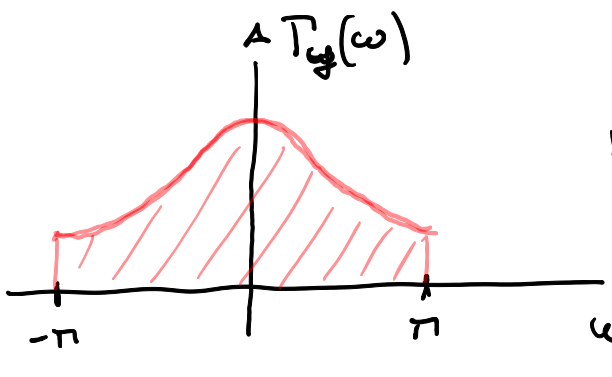
\includegraphics[width=.5\linewidth]{varspec}
\end{figure}
\end{description}
\newpage
\subsection{White Noise in the frequency domain}
In case we are dealing with a WN : $ e(t) = WN(0,\lambda^2)$ we can consider it in three different domains.
\begin{enumerate}
\item \textbf{Time domain}\\
WN is clearly \textbf{unpredictable}
\begin{figure}[H]
 \centering
  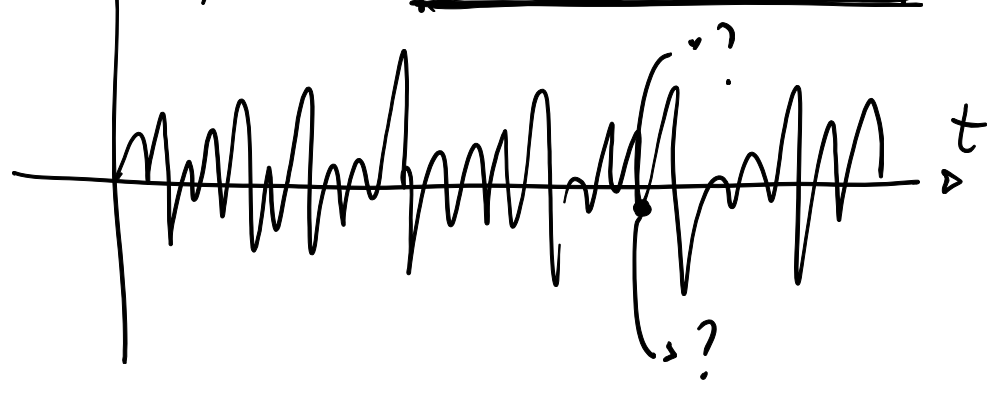
\includegraphics[width=.4\linewidth]{unpredic}
\end{figure}

\item \textbf{Probabilistic domain}\\
Considering the WN in the probabilistic domain and plotting its \textbf{variance} only $ \gamma_e(0) \neq 0 $ : there is no \textbf{correlation} between $ e(t) $ and $ e(t \pm \tau) $ 
\begin{figure}[H]
 \centering
  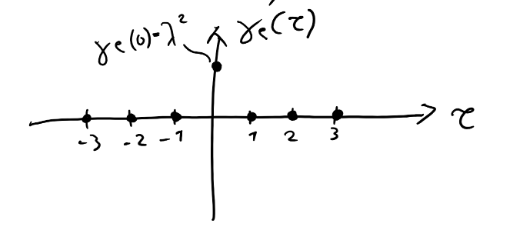
\includegraphics[width=.4\linewidth]{no_cov}
\end{figure}
\item \textbf{Frequency domain}\\
Since the definition of FT relies on the definition of \textbf{covariance} $ \gamma_e(\tau) $ , as seen in point 2 only for $ \tau = 0 \to \gamma_e(\tau) \neq 0$ : 
\[
\boxed{\Gamma_e(w) = \gamma_e(0)e^{jw0} = \gamma_e(0) = \lambda^2}
\]
\begin{figure}[H]
 \centering
  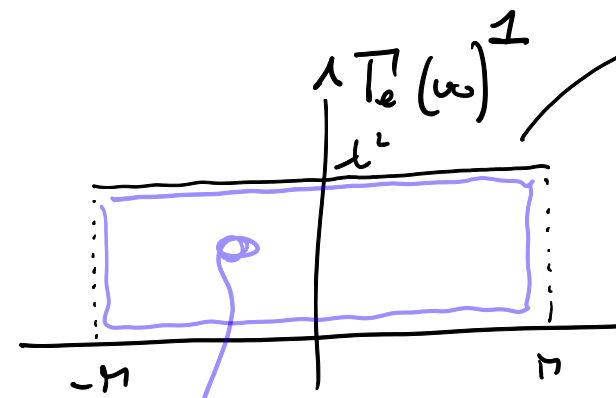
\includegraphics[width=.4\linewidth]{ftwn}
\end{figure}
The area is $ 2\pi\lambda^2$  so the variance is $ \frac{area}{2\pi} = \lambda^2 = \gamma_e(0)$\\
The \textbf{energy} of the WN is \textbf{uniformly distributed} over all frequencies.
\end{enumerate}

\subsection{Computation of the spectrum of a process generated as the output of a digital system}
Problem : the \textbf{computation} of the $\Gamma_y(w)$ is quite difficult most of the times. A \textbf{simpler} alternative can be found using the notion of \textbf{Frequency Response}.

\subsubsection{Frequency Response of a linear system}
Given two signals (\textbf{SSP}) input v(t) and output y(t) , where input passes through W(Z) the system or digital filter , then the \textbf{frequency response} is 
$$ W(e^{jw})$$ which corresponds to the evaluation of the \textbf{transfer function} on the \textbf{unit circumference } 
\begin{figure}[H]
 \centering
  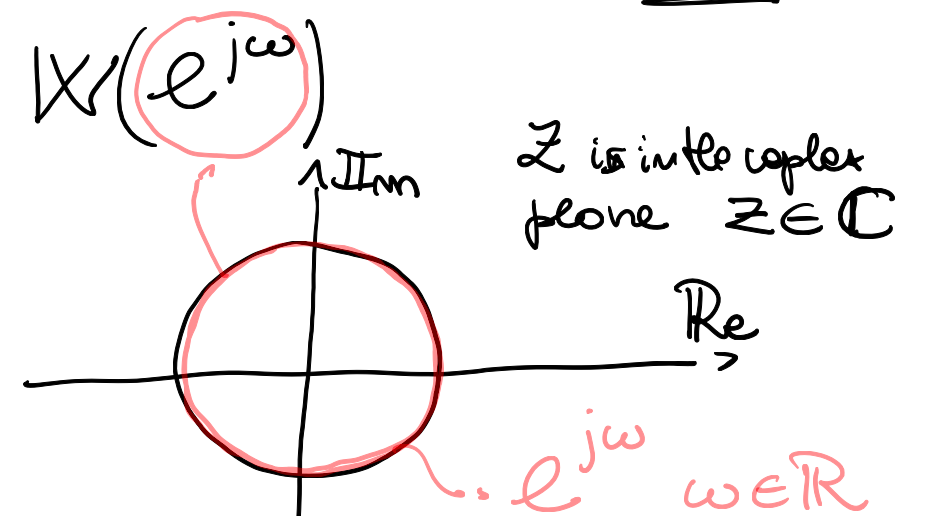
\includegraphics[width=.3\linewidth]{tf_fr}
\end{figure}
The frequency response is used in system theory in the \textbf{Frequency Response Theorem}
\begin{description}
\item[FR Th.]\hfill\\
If W(Z) is \textbf{asymptotically stable} and v(t) is $Asen(\Omega t + \phi $ , where
A is the amplitude an $\phi$ the phase of the sinusoid , the the output is a \textbf{pure sinusoid} with :
\newpage
\begin{itemize}
\item the \textbf{same} angular speed $\Omega$
\item amplitude $A|W(e^{j\Omega})| \to$  \textbf{gain}
\item phase $\phi +\angle W(e^{j\Omega})\to $ \textbf{shift in phase}
\end{itemize}
\[
 \boxed{y(t) =A|W(e^{j\Omega})| sen(\Omega t + \phi + \angle W(e^{j\Omega}) }
\]

\begin{figure}[H]
 \centering
  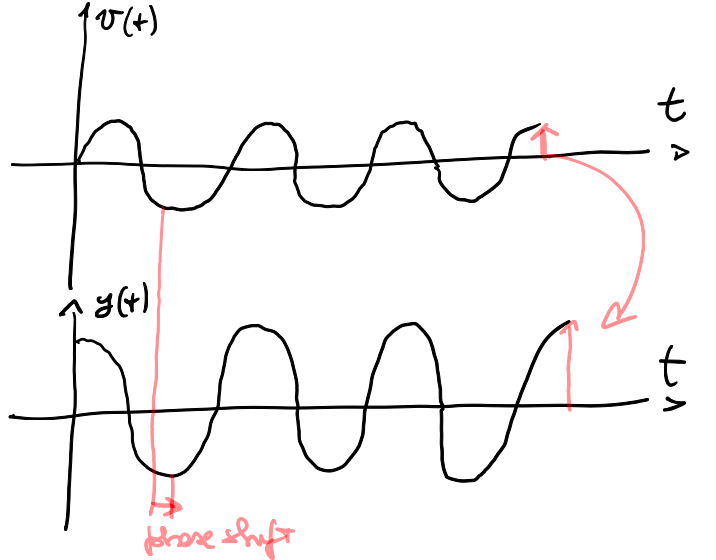
\includegraphics[width=.4\linewidth]{FRgraph}
\end{figure}

\item[1.FR Nyquist plot]\hfill\\
$W(e^{jw})$ is a complex function of a \textbf{real} variable.\\
\begin{figure}[H]
 \centering
  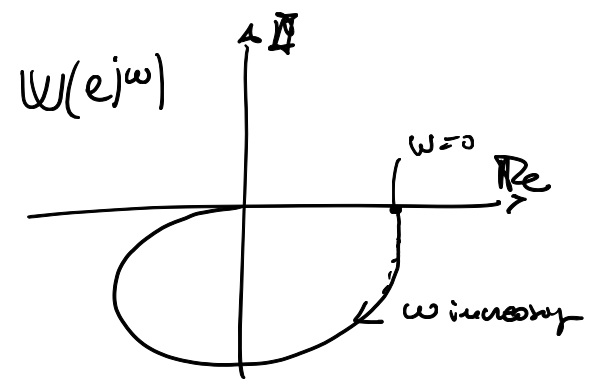
\includegraphics[width=.4\linewidth]{nqplot}
\end{figure}
\newpage
\item[2.FR Bode plot]\hfill\\
Bode plot gives information about \textbf{magnitude} and \textbf{phase}
\begin{figure}[H]
 \centering
  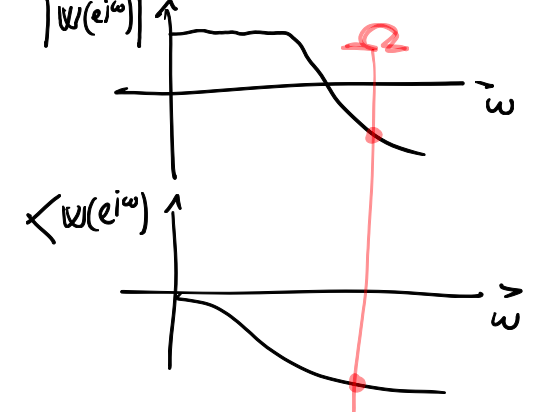
\includegraphics[width=.4\linewidth]{bodeplot}
\end{figure}
\end{description}

\subsubsection{Spectrum computation with FR}
If y(t) is output of a transfer function W(Z) which is \textbf{asymptotically stable} with input signal v(t) , then the spectrum is:
\[
 \boxed{ \Gamma_y(w) = |W(e^{jw})|^2 \Gamma_v(w)}
\]

The computation of $\Gamma_v(w)$ still remains but most of the time signal v(t) is a \textbf{white noise} $\sim (0,\lambda^2)$ which means that $\Gamma_v(w) = \lambda^2$


\subsection{Equivalent representations of ARMA}
An ARMA SSP can be represented in 4 different but \textbf{equivalent} ways with $e(t) 
\sim WN(0,1)$:
\begin{enumerate}
\item \textbf{Time domain} $ y(t) = a_1y(t-1)+...+a_my(t-m) +c_0e(t)+...+c_ne(t-n)$
\item \textbf{Transfer function} $ y(t) = \frac{C(Z)}{A(Z)} e(t) $
\item \textbf{Probabilistic domain}:
 \[  
  \begin{cases}
    m_y       & \quad = E[y(t)]\\
    \gamma_y(\tau)  & \quad =  E[(y(t)-m_y)(y(t-\tau)-m_y)]
  \end{cases}
\]
\item \textbf{Frequency domain} 
 \[  
  \begin{cases}
    m_y       & \quad = E[y(t)]\\
    \Gamma_y(w)  & \quad w \in \Re
  \end{cases}
\]
\end{enumerate}

\begin{figure}[H]
 \centering
  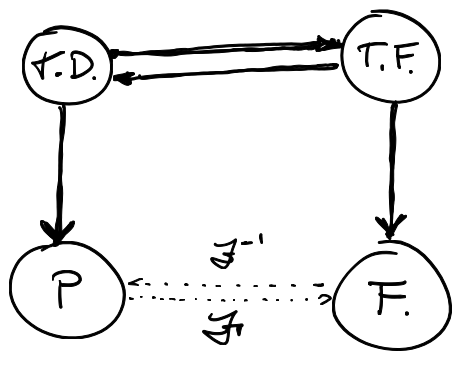
\includegraphics[width=.4\linewidth]{domainscheme}
  \caption{Bold : usual transformation , dotted : feasible but difficult}
\end{figure}

\subsection{Example \& Exercises }
\begin{description}
\item[Example 1]\hfill\\
Given 3 output spectra match the corresponding time domain representation.
\begin{figure}[H]
 \centering
  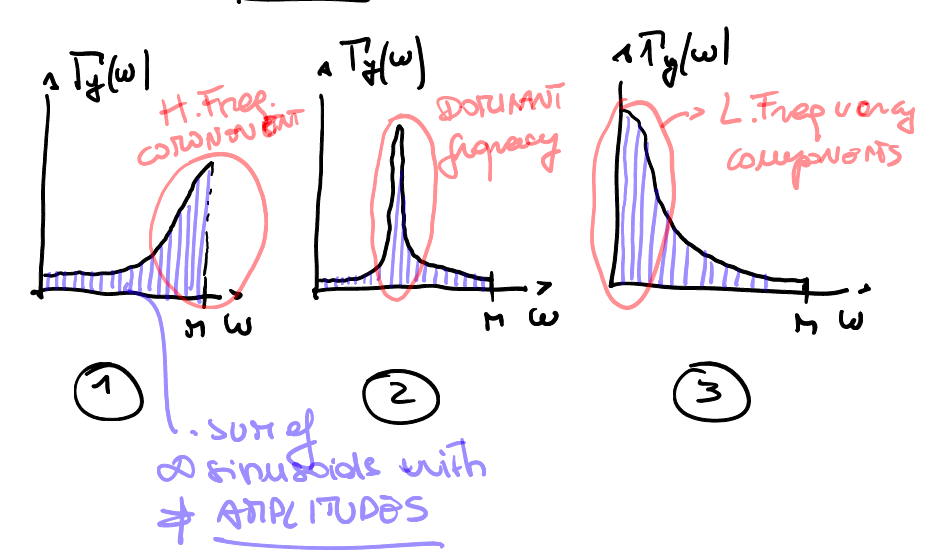
\includegraphics[width=.4\linewidth]{ex1_q}
\end{figure}
\begin{figure}[H]
 \centering
  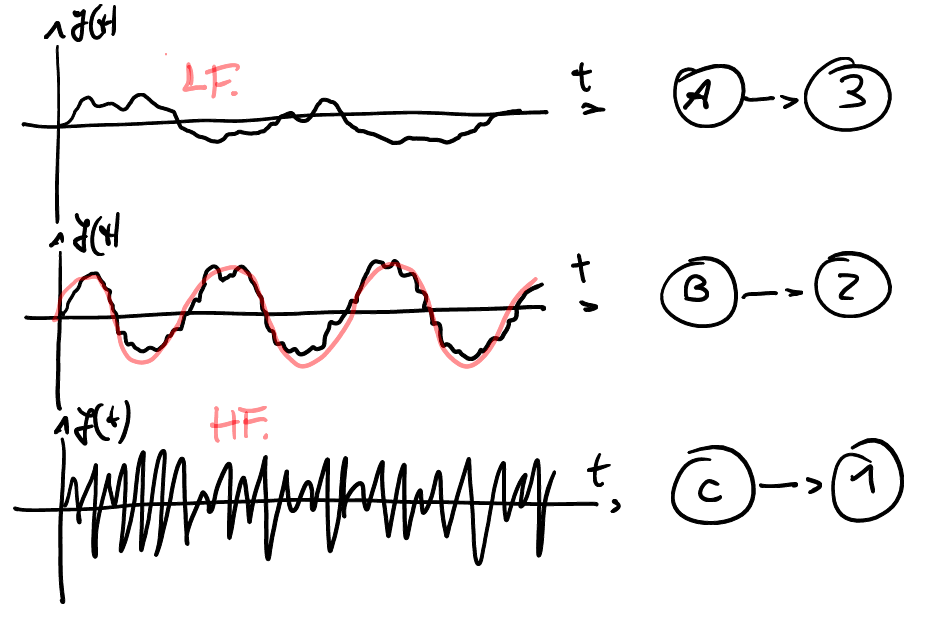
\includegraphics[width=.4\linewidth]{ex1_s}
\end{figure}

\newpage
\item [Example 2]\hfill\\
Given a \textbf{MA(1)} process $ y(t)= e(t) + ce(t-1)  , e \sim WN(0,\lambda^2) , c \in \Re$.
- y(t) is \textbf{stationary} because MA(1) is always \textbf{asymptotically stable}
- $m_e = 0 \to m_y = 0 $
- $\gamma_y(0) = \lambda^2(1+c^2) $
- $\gamma_y(1) = \lambda^2c $
- $ \gamma_y(\tau) = 0 , |\tau| \geq 2 $
\begin{figure}[H]
 \centering
  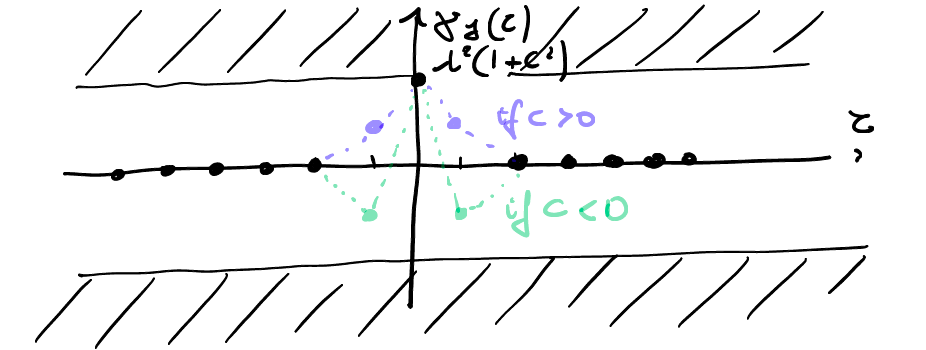
\includegraphics[width=.5\linewidth]{ex2_g}
\end{figure}
1.Composition of $\Gamma_y(w)$ with $\lambda^2 = 1$:
\begin{itemize}
\item \textbf{From definition}\\
$$ \Gamma_y(w) = \sum\limits_{\tau = -\infty}^{\infty} \gamma_y(\tau)e^{-jw\tau} $$ 
- For $\tau =0 :(1+c^2) $\\
- For $\tau =1 : ce^{-jw} $\\
- For $\tau =-1 : c+e^{+jw}$\\
- For $|\tau| \geq 2 : 0 $
$$ \Gamma_y(w) = 1+c^2 + c(e^{-jw}+e^{+jw})$$
Recall : $ e^{-jw} + e^{jw} = cosw - jsenw + cosw + jsenw = 2cosw $
$$ \Gamma_y(w) = (1+c^2) + 2c cosw $$
Which is \textbf{real, positive, even , periodic}
\item \textbf{From frequency response}\\
The MA(1) transfer function is $$ y(t) = (1+cZ^{-1})e(t) $$
$$ \Gamma_y(w) = |W(e^{jw}|^2\Gamma_e(w) = |1+ce^{-jw}|^2 \cdot 1 $$
Recall : $ |a+jb|^2 = Im[a+ib]^2+Re[a+ib]^2 = a^2+b^2 = (a+jb)(a-jb) $
$$ (1+ce^{-jw})(1-ce^{jw}) = 1+c^2(e^{jw} \cdot e^{-jw})+c(e^{-jw}+e^{jw}) = 1+c^2+2c cosw $$
2.Plotting of $ \Gamma_y(w)$ : \\
$ \Gamma_y(0) = (1+c)^2 $\\
$ \Gamma_y(\frac{\pi}{2} = 1+c^2)$\\
$ \Gamma_y(\pi) = (1-c)^2 $
\begin{figure}[H]
 \centering
  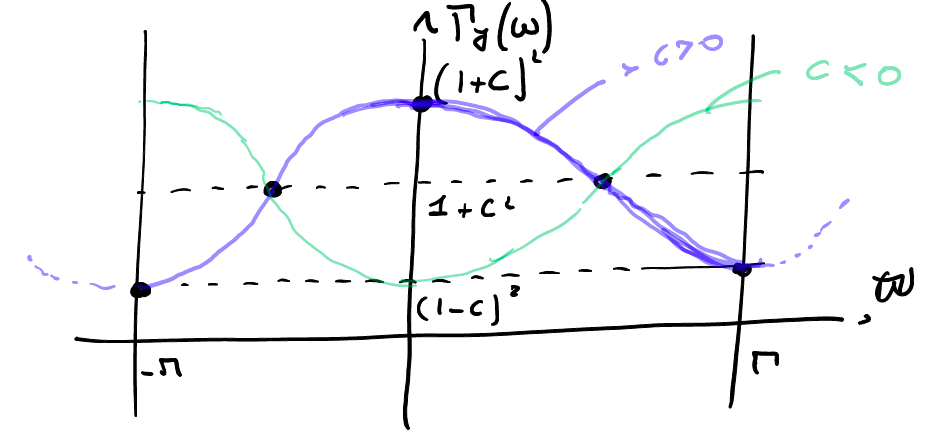
\includegraphics[width=.7\linewidth]{ex2_p}
\end{figure}
3.Compute the variance $\gamma_y(0)$ given $\Gamma_y(w)$ :
$$ \gamma_y(0) = \frac{1}{2\pi} \int_{-\pi}^{\pi} \Gamma_y(w)dw = \frac{1}{2\pi} \int_{-\pi}^{\pi}(1+c^2 +2ccosw) dw $$ 
$$ \frac{1}{2\pi} \int_{-\pi}^{\pi}(1+c^2)dw + \frac{1}{2\pi} \int_{-\pi}^{\pi} 2ccosw dw $$ $$ \frac{1}{2\pi} [(1+c^2) [w]_{-\pi}^{\pi} + 2c[senw]_{-\pi}^{\pi}] = \frac{1}{2\pi}[(1+c^2)(2\pi)] = $$ $$ 1+c^2$$ 
\end{itemize}
\newpage
\item [Example 3]\hfill\\
\begin{figure}[H]
 \centering
  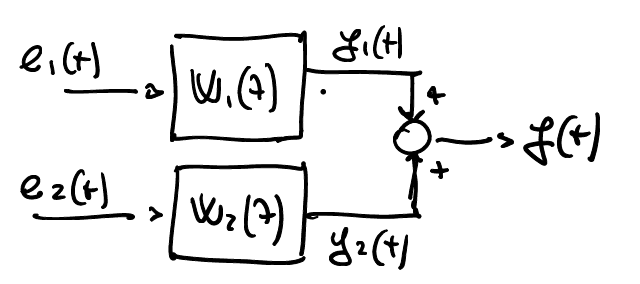
\includegraphics[width=.5\linewidth]{ex3_g}
\end{figure}
Consider the SSP y(t) generated by 2 inputs.\\
$W_1(t),W_2(t)$ are asymptotically stable.\\
$ e_1(t) \sim W(0,\lambda_1^2) , e_2(t) \sim W(0,\lambda_2^2) $\\
$ e_1 \perp e_2 \to E[e_1(t)e_2(t-\tau)]=0$\\
Calculate $\gamma_y(\tau)$ and $\Gamma_y(w)$
\begin{itemize}
\item $\gamma_y(\tau)$\\
$\gamma_y(\tau) = E[y(t)y(t-\tau)] = E[(y_1(t)+y_2(t))(y_1(t-\tau)+y_2(t-\tau))]$\\
$ E[y_1(t)y_1(t-\tau)] + E[y_2(t)y_2(t-\tau)] + E[y_1(t)y_2(t-\tau)] + E[y_2(t)y_1(t-\tau)] $ \\
$ \gamma_{y_1}(\tau) + \gamma_{y_2}(\tau) + 0 + 0 $ \\
Term 3 and 4 are = 0 which is a result obtained by rewriting them as $MA(\infty)$ and exploiting the hypothesis that $e_1(t) \perp e_2(t)$.
\[
\boxed{\gamma_y(t)= \gamma_{y_1}(t) + \gamma_{y_2}(t)}
\]
\item $\Gamma_y(t)$\\
$\Gamma_y(t) = \sum\limits_{\tau = -\infty}^{\infty} \gamma_y(\tau)e^{-jw\tau} =
\sum\limits_{\tau = -\infty}^{\infty} \gamma_{y_1}(\tau)e^{-jw\tau} + \sum\limits_{\tau = -\infty}^{\infty} \gamma_{y_2}(\tau)e^{-jw\tau} $ \\ 
\[
\boxed{\Gamma_y(w)=\Gamma_{y_1}(w) + \Gamma_{y_2}(w)}
\]
\end{itemize}
The result can be generalised to more than 2 inputs that are summed to form an SSP y(t): 
\[
\boxed{\gamma_y(t)= \gamma_{y_1}(t) + \gamma_{y_2}(t) +...+ \gamma_{y_k}(t) }
\]
\[
\boxed{\Gamma_y(w)= \Gamma_{y_1}(w) + \Gamma_{y_2}(w) +...+ \Gamma_{y_k}(t) }
\]
The result hold if all $W_i(t)$ are asymptotically stable , all $v_i(t)$ are ssp and incorrelated
\item[Example 4]\hfill\\
Consider the following AR(1) SSP $y(t) = \frac{1}{3}y(t-1)+e(t)+2 \to e \sim WN(1,1)$
which has a asymptotically stable TF.\\
Calculate $m_y$ and $\gamma_y$.\\
\begin{itemize}
\item \textbf{Mean of y}\\
\begin{itemize}
\item \textbf{Method 1}\\
$E[y(t)] = E[\frac{1}{3}y(t-1)e(t)+2] \to (1-\frac{1}{3})m_y = m_e+2 \to m_y = \frac{9}{2}$
\item \textbf{Mehotd 2}\\
\begin{figure}[H]
 \centering
  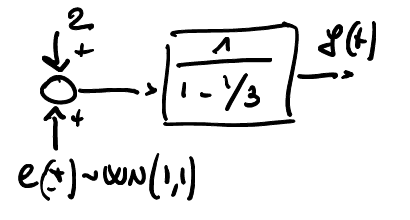
\includegraphics[width=.4\linewidth]{ex4_g}
\end{figure}
$e(t) = \tilde{e} +1 , \tilde{e} \sim WN(0,1)$\\
Using the superposition principle of LTI systems :
\begin{figure}[H]
 \centering
  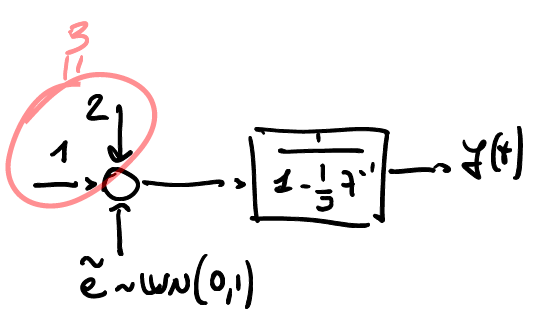
\includegraphics[width=.4\linewidth]{ex4_g2}
\end{figure}
\begin{figure}[H]
 \centering
  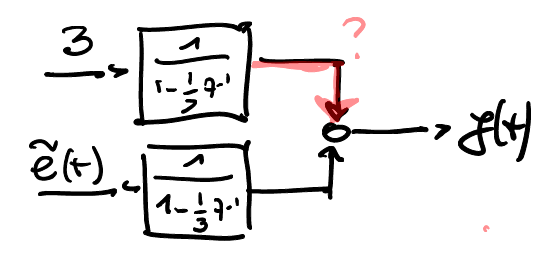
\includegraphics[width=.4\linewidth]{ex4_g3}
\end{figure}
The constant value 3 can be seen as a \textbf{sinusoidal signal with w=0} so the \textbf{Frequency Response Theorem } can be applied: \\
$ 3(\frac{1}{1-\frac{1}{3}Z^{-1}}) \text{calculated in} z=e^{j0}$ \\
$ 3(\frac{1}{1-\frac{1}{3}}) = \frac{9}{2}$
And since $m_{\tilde{e}}$ is a zero mean signal $\to m_y = \frac{9}{2}$
\end{itemize}
\item \textbf{Covariance of y}\\
\begin{itemize}
\item \textbf{Method 1 : BAD}\\
$ E[(y(t)-\frac{9}{2})^2] = E[(\frac{1}{3}y(t-1)+e(t)+2-\frac{9}{2})^2]$\\
$ \gamma_y(0) = \frac{1}{9}E[y(t-1)^2]+E[e(t)^2]+\frac{25}{4} + \frac{2}{3}E[y(t-1)e(t)]-\frac{5}{3}E[y(t-1)]+5E[e(t)]$\\
------------------------------------------------------------------------------------\\
\textbf{Remark:} $E[(e(t)-m_e) = \gamma_e(0) =E[e(t)^2]-2E[e(t)m_e] + m_e^2$ \\ 
$E[e(t)]= \gamma_e(0) + m_e^2$ \\
Which can be generalised : \\
\[
\boxed{E[e(t)^2]= \gamma_e(0)+m_e^2}
\]
\[
\boxed{E[y(t)^2]= \gamma_y(0)+m_y^2}
\] 
$E[e(t)y(t-1)]= E[(e(t)-m_e)(y(t-1)-m_y)]+m_ym_e$
\[
\boxed{E[e(t)y(t-1)]= m_em_y}
\]
As the \textbf{de-biased signals are incorellated!}\\
------------------------------------------------------------------------------------\\
$\gamma_y(0) = \frac{1}{9}(\gamma_y(0)+m_y^2)+(\gamma_e(0) + m_e^2)+ \frac{25}{4} + \frac{2}{3}(m_em_y)-\frac{5}{3}m_y-5m_e = \frac{9}{8}$
Same computations for $\gamma_y(1),\gamma_y(2)...$
\item \textbf{Method 2: GOOD}\\
Define two new processes: \\
$ \tilde{y}(t) = y(t) - \frac{9}{2} \to m_{\tilde{y} = 0}$\\
$ \tilde{e}(t) = e(t) - 1 \to m_{\tilde{e}=0}$\\
So $ y(t) = \tilde{y}(t) - \frac{9}{2} $ and $ e(t) = \tilde{e}(t) + 1$  : \\
$ \tilde{y}(t)+\frac{9}{2} = \frac{1}{3}(\tilde{y}(t-1)+\frac{9}{2}) + (\tilde{e}+1)+2$
\[
\boxed{\tilde{y}(t) = \frac{1}{3}\tilde{y}(t-1)+\tilde{e}(t), \tilde{e} \sim WN(0,1)}
\]
Where $\tilde{y}(t)$ is the \textbf{de-biased process}\\
$\gamma_{\tilde{y}(0)} = \frac{1}{1-\frac{1}{9}} = \frac{9}{8}$\\
$\gamma_{\tilde{y}(1)} = \frac{9}{8}\frac{1}{3} = \frac{3}{8}$\\
$\gamma_{\tilde{y}(2)} = \frac{3}{8}\frac{1}{3} = \frac{1}{8}$   ...\\
Now that we found $\gamma_{\tilde{y}(\tau)}$ we want to find $\gamma_y(\tau)$
$ \gamma_y(\tau) $: \\$E[(y(t)-\frac{9}{2})(y(t-\tau)-\frac{9}{2})] = E[\tilde{y}(t)\tilde{y}(t-\tau)]=\gamma_{\tilde{y}}(\tau)$  \\ since $m_{\tilde{y}}=0$
Which can be generalised :\\
If  $y(t)$ and $\tilde{y(t)}$ are two SSPs that \textbf{differ only from a constant value} $y(t) = \tilde{y}(t)+k$ then :
\[
\boxed{\gamma_y(\tau)= \gamma_{\tilde{y}} , \forall \tau}
\]
\[
\boxed{\Gamma_y(w)= \Gamma_{\tilde{y}} ,\forall w}
\]
\end{itemize}
\end{itemize}
\end{description}
